\documentclass[12pt]{article}
 
\usepackage[margin=1in]{geometry}
\usepackage{amsmath,amsthm,amssymb}
\usepackage{graphicx}
\graphicspath{ {Images/} }
\usepackage{listings}
\usepackage{color}
\definecolor{light-gray}{gray}{0.92}

\newcommand{\N}{\mathbb{N}}
\newcommand{\R}{\mathbb{R}}
\newcommand{\Z}{\mathbb{Z}}
\newcommand{\Q}{\mathbb{Q}}
 

\newenvironment{problem}[2][Problem]{\begin{trivlist}
\item[\hskip \labelsep {\bfseries #1}\hskip \labelsep {\bfseries #2.}]}{\end{trivlist}}


\begin{document}
\title{\textsc{EN.553.732 (STAT 732)} Homework 4}
\author{\textsc{Joseph High} \ -- \ \textsc{Hopkins ID: 9E1FDC}}
\date{\today}
\maketitle

\begin{problem}{1} \textit{Problem 9.2 from Hoff}
\\\
\\\
\textbf{Part a} 
\\\
Using a g-prior with $g=n$, $\nu_0=2$ and $\sigma_0^2=1$, a regression model was fit and the posterior confidence intervals for the parameters were computed (provided in Table 1 below). The plots of the posterior distributions were also computed (blue lines are 95\% confidence intervals) 
\\\
\\\
\textbf{R Code} 
\lstset{backgroundcolor=\color{light-gray}, frame=single, basicstyle = \ttfamily\small}
\begin{lstlisting}{language=R}
#Problem 1 Part a
set.seed(1)
t=10000
azdiabetes = read.table("azdiabetes.dat", header = TRUE);
y=as.matrix(azdiabetes[,2])
g=length(y)
X=as.matrix(cbind(rep(1,g),azdiabetes[,-c(2,8)]))
n=nrow(X)
m=ncol(X)
nu_0=2
sigma2_0=1
Hg=(g/(g+1))*X%*%solve(t(X)%*%X)%*%t(X)
SS=t(y)%*%(diag(1,nrow=n)-Hg)%*%y
sigma2=1/rgamma(t,(nu_0+n)/2,(nu_0*sigma2_0+SS)/2)
Vb=g*solve(t(X)%*%X)/(g+1)
Eb=Vb%*%t(X)%*%y
E=matrix(rnorm(t*m,0,sqrt(sigma2)),t,m)
b=t(t(E%*%chol(Vb))+c(Eb))
for (i in 1:m) 
{
  print(quantile(b[,i],c(0.025, 0.975)))
}         
plot(density(b[,2]),col=1, xlab=names(azdiabetes)[1], 
main ="Problem 1 Part a")
abline(v=mean(b[,2]),col=2)
abline(v=quantile(b[,2],0.025),col=4)
abline(v=quantile(b[,2],0.975),col=4)
for (i in 2:6) 
{
  plot(density(b[,i+1]),col=1, xlab=names(azdiabetes)[i+1], 
  main ="Problem 1 Part a")
  abline(v=mean(b[,i+1]),col=2)
  abline(v=quantile(b[,i+1],0.025),col=4)
  abline(v=quantile(b[,i+1],0.975),col=4)
}
\end{lstlisting}

\begin{table}[h]
\centering
\caption{Posterior Confidence Intervals}
\label{my-label}
\begin{tabular}{|l|l|}
\hline
& 95\% CI \\ \hline
Intercept & (35.083, 69.244)    \\ \hline
\texttt{npreg}       & (-1.625, 0.304)  \\ \hline
\texttt{bp}          & (-0.0207, 0.429) \\ \hline
\texttt{skin}        & (-0.122, 0.504)  \\ \hline
\texttt{bmi}         & (0.161, 1.141)  \\ \hline
\texttt{ped}         & (3.159, 17.923)  \\ \hline
\texttt{age}         & (0.456, 1.080)  \\ \hline
\end{tabular}
\end{table}

\textbf{Posterior distribution plots} \textit{Blue lines correspond to the 95\% confidence intervals}
\\\
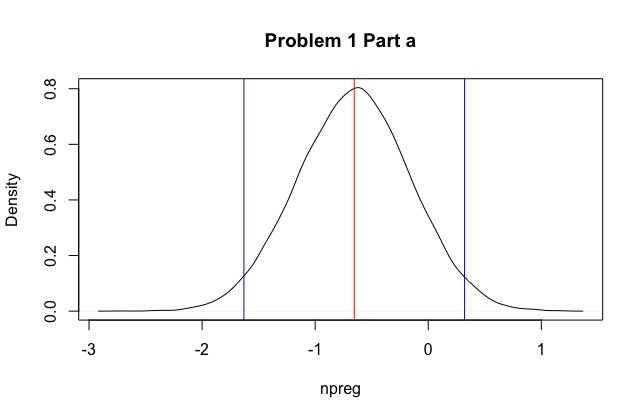
\includegraphics[width=8cm,height=8cm,keepaspectratio]{1a1.jpeg}
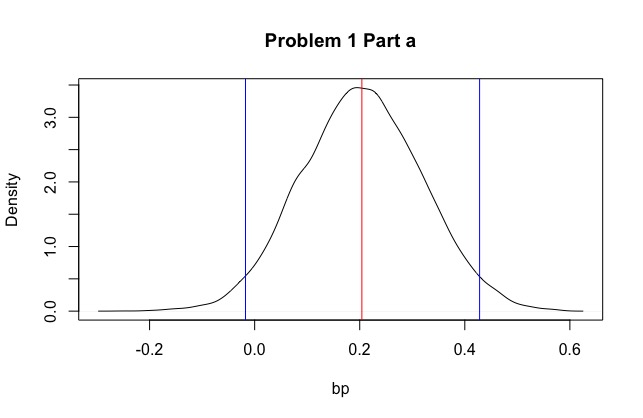
\includegraphics[width=8cm,height=8cm,keepaspectratio]{1a2.jpeg}\\
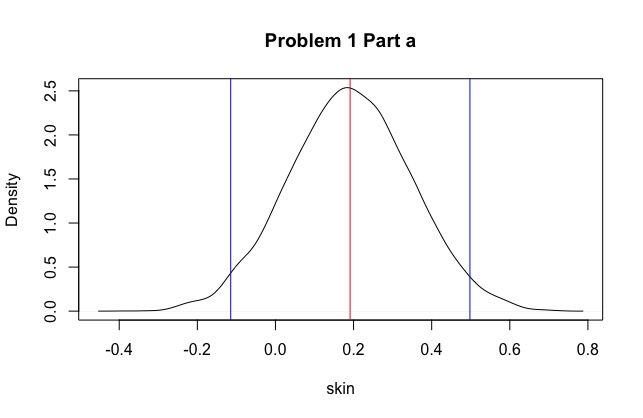
\includegraphics[width=8cm,height=8cm,keepaspectratio]{1a3.jpeg}
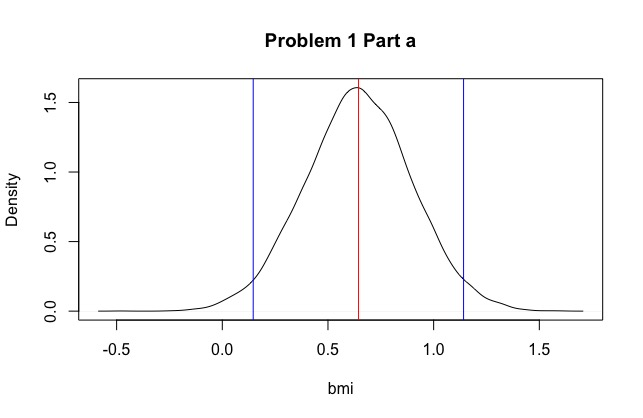
\includegraphics[width=8cm,height=8cm,keepaspectratio]{1a4.jpeg}\\
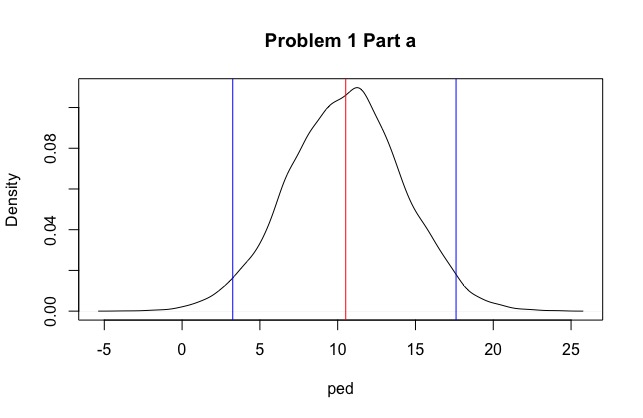
\includegraphics[width=8cm,height=8cm,keepaspectratio]{1a5.jpeg}
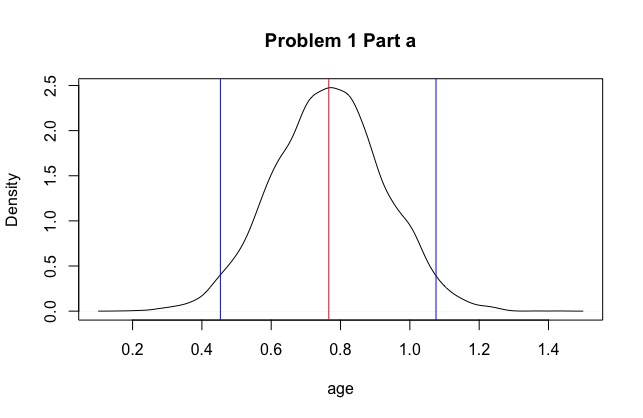
\includegraphics[width=8cm,height=8cm,keepaspectratio]{1a6.jpeg}\\
\\
\\\
\textbf{Part b}
\\\
Now, we perform the model selection process and the averaging procedure using the same g-prior. Table 2 below summarizes the results for $Pr(\beta_j\neq0|y)$ and the posterior confidence intervals for all parameters. The plots below are the posterior distributions for the parameters, and the blue lines are the 95\% confidence intervals. Comparing the results from part a and b, we see that for the \texttt{npreg}, \texttt{bp}, and \texttt{skin} parameters, their respective 95\% posterior confidence intervals include 0 for in part b. The value of $Pr(\beta_j\neq0|y)$ for these three parameters are all close to 0, and their posterior distributions are more narrow than in part a. For the other parameters, where $Pr(\beta_j\neq0|y)$ is close to 1, the confidence intervals are not significantly different from their confidence intervals in part a. \\
\\\
\textbf{R Code} 
\\\
\lstset{backgroundcolor=\color{light-gray}, frame=single, basicstyle = \ttfamily\small}
\begin{lstlisting}{language=R}
#Problem 1 Part b
lpy.X=function(y, X) 
{
  n=nrow(X)
  m=ncol(X)
  g=length(y)
  nu_0=1
  sigma2_0=try(summary(lm(y ~ -1+X))$sigma^2, silent = TRUE)
  if (m == 0) 
  {
    Hg=0
    sigma2_0=mean(y^2)
  }
  else if (m > 0) 
  {
    Hg=(g/(g+1))*X%*%solve(t(X)%*%X)%*%t(X)
  }
  SS=t(y)%*%(diag(1, nrow = n)-Hg)%*%y
  -(1/2)*(n*log(pi)+m*log(1+g)+(nu_0+n)*log(nu_0*sigma2_0+SS)-
  nu_0*log(nu_0*sigma2_0))+lgamma((nu_0+n)/2)-lgamma(nu_0/2)
}
t=1000
A=matrix(NA, t, m)
B=matrix(0, t, m)
a=rep(1, m)
lpy.c=lpy.X(y, X[, a == 1, drop = FALSE])
for(i in 1:t) 
{
  for(j in sample(1:m)) 
  {
    temp=a
    temp[j]=1-temp[j]
    lpy.m=lpy.X(y, X[, temp == 1, drop = FALSE])
    r=(lpy.m-lpy.c)*(-1)^(temp[j] == 0)
    a[j]=rbinom(1, 1, 1/(1+exp(-r)))
    if (a[j] == temp[j]) 
    {
      lpy.c=lpy.m
    }
    A[i, ]=a
    Hg=(g/(g+1))*X[, A[i,] == 1, drop = FALSE]%*%solve(t(X[, 
    A[i,] == 1, drop = FALSE])%*%X[, A[i,] == 1, 
    drop = FALSE])%*%t(X[, A[i,] == 1, drop = FALSE])
    SS=t(y)%*%(diag(1, nrow = n)-Hg)%*%y
    sigma2=1/rgamma(t, (nu_0+n)/2, (nu_0*sigma2_0+SS)/2)
    Vb=g*solve(t(X[, A[i,] == 1, drop = FALSE])%*%X[, A[i,] == 1, 
    drop = FALSE])/(g+1)
    Eb=Vb%*%t(X[, A[i,] == 1, drop = FALSE])%*%y
    E=matrix(rnorm(sum(A[i, ]), 0, sqrt(sigma2)), 1, sum(A[i, ]))
    B[i, A[i,] == 1]=t(t(E%*%chol(Vb))+c(Eb))
  }
}
for (i in 1:m) 
{
  print(sum(B[,i]!= 0)/t)
}
for (i in 1:m) 
{
  print(quantile(B[,i],c(0.025, 0.975)))
}         
plot(density(B[,2]),col=1, xlab=names(azdiabetes)[1], 
main ="Problem 1 Part b")
abline(v=mean(B[,2]),col=2)
abline(v=quantile(B[,2],0.025),col=4)
abline(v=quantile(B[,2],0.975),col=4)
for (i in 2:6) 
{
  plot(density(B[,i+1]),col=1, xlab=names(azdiabetes)[i+1], 
  main ="Problem 1 Part b")
  abline(v=mean(B[,i+1]),col=2)
  abline(v=quantile(B[,i+1],0.025),col=4)
  abline(v=quantile(B[,i+1],0.975),col=4)
}
\end{lstlisting} 
\textbf{Output:}
\begin{table}[h]
\centering
\caption{Problem 1 Part b}
\label{my-label}
\begin{tabular}{|l|l|l|}
\hline
& $Pr(\beta_j\neq0|y)$ & 95\% CI \\ \hline
(Intercept) & 1             &  (42.650, 76.874)     \\ \hline
\texttt{npreg}       &  0.149             & (-1.1151, 0.000)   \\ \hline
\texttt{bp}          &    0.291          & (0.000, 0.369)    \\ \hline
\texttt{skin}       &  0.158            &  (0.000, 0.411)     \\ \hline
\texttt{bmi}         &   0.989           &  (0.469, 1.347)    \\ \hline
\texttt{ped}         &     0.899         &( 0.000, 17.561)  \\ \hline
\texttt{age}         &      1         & (0.480, 0.993)   \\ \hline
\end{tabular}
\end{table}
\\\
\textbf{Posterior distribution plots} \textit{Blue lines correspond to the 95\% confidence intervals}
\\\
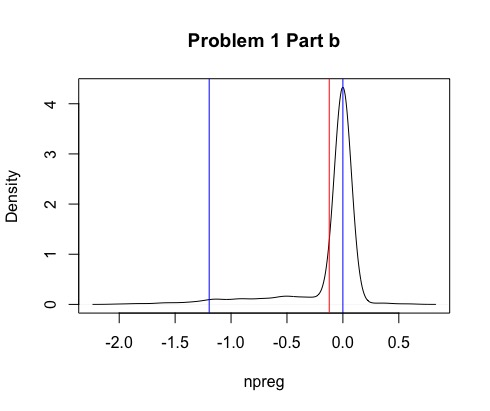
\includegraphics[width=8cm,height=8cm,keepaspectratio]{1b1.jpeg}
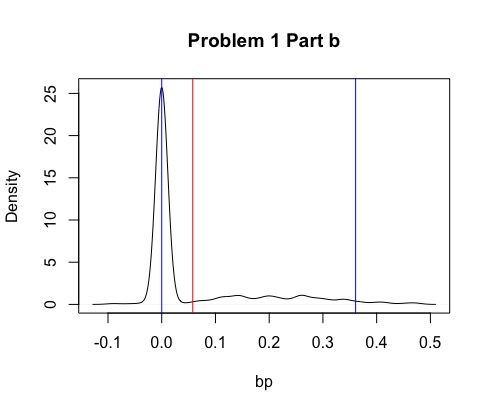
\includegraphics[width=8cm,height=8cm,keepaspectratio]{1b2.jpeg}\\
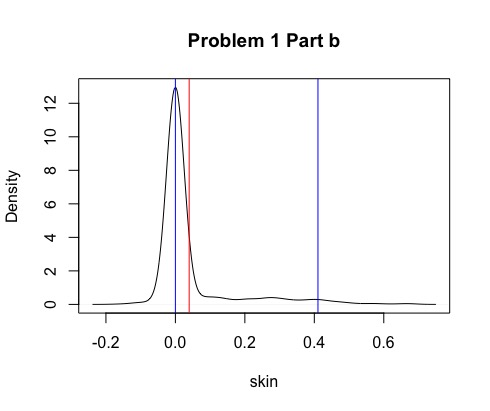
\includegraphics[width=8cm,height=8cm,keepaspectratio]{1b3.jpeg}
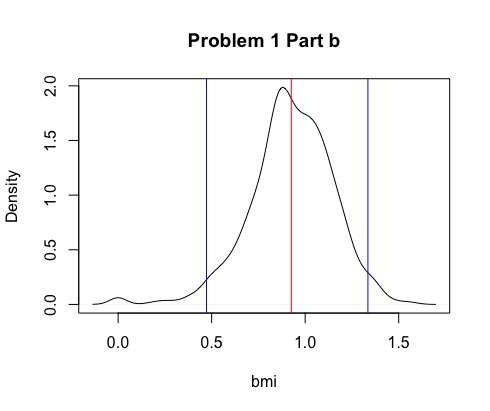
\includegraphics[width=8cm,height=8cm,keepaspectratio]{1b4.jpeg}\\
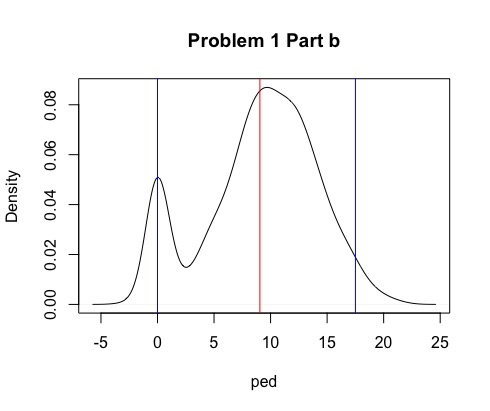
\includegraphics[width=8cm,height=8cm,keepaspectratio]{1b5.jpeg}
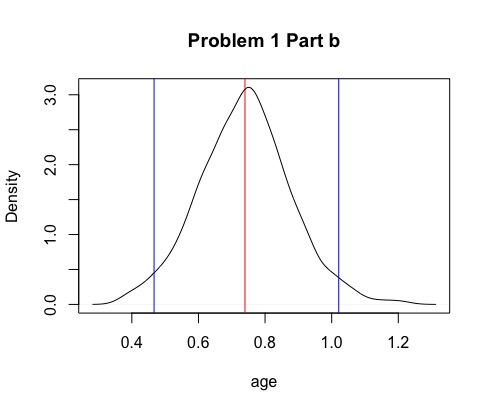
\includegraphics[width=8cm,height=8cm,keepaspectratio]{1b6.jpeg}\\

\end{problem}

\begin{problem}{2} \textit{Problem 9.3 from Hoff}
\\\
\\\
\textbf{Part a}
\\\
We fit the regression model using the g-prior with $g=47$, $v_{0}=2$, and $\sigma_{0}^{2}=1$. 
The left side of the table below gives the marginal posterior means and confidence intervals for all the variables. The right side gives the summary of the least squares estimates for each variable, with the mean, confidence interval, and p-values. Comparing the two sides of the table, we can see that the confidence intervals for the least squares approach is generally wider than that for the Bayesian approach. But their means are rather similar. The plots for the posterior distributions for each variable is also give below, with the means (blue) and 95\% confidence intervals (green). The R code is also shown below\\
\\\
There are a couple of ways to determine whether a variable is strongly predictive of crime rates. If 0 is not contained in its $95\%$ confidence interval, by the Bayesian approach, then it implies that it has a noticeable effect on crime rates. Another indicator of significant effect on crime rate is the p-value. From the least squares approach, if the p-value is small, it has a significant effect on the crime rate. Both methods were used (denoted by * in Table 3). \\
\\\
It is seen that the strong predictors of crime rates are \texttt{M} (percentage of males aged 14 − 24), \texttt{Ed} (mean years of schooling), \texttt{U2} (unemployment rate of urban males 3539), \texttt{Ineq} (income inequality), and \texttt{Prob} (probability of imprisonment). Two of the variables with the lowest p-values are \texttt{Ed} and \texttt{Ineq}. They are the two most significant positively-correlated variables with crime rates. The most significant negatively-correlated variable is \texttt{Prob}, which is intuitively clear. Indeed, a higher probability of imprisonment usually leads to lower crime rates.\\
\\\
\textbf{R Code} 
\\\
\lstset{backgroundcolor=\color{light-gray}, frame=single, basicstyle = \ttfamily\small}
\begin{lstlisting}{language=R}
#Problem 2 Part a
crime = read.table("crime.dat", header = TRUE)
y = as.matrix(crime[,1])
X = as.matrix(cbind(rep(1, dim(y)[1], 1),crime[,-1]))
g = length(y)
nu_0 = 2
sigma2_0 = 1
n = dim(X)[1]
m = dim(X)[2]
t = 10000
Hg = (g/(g+1))*X%*%solve(t(X)%*%X)%*%t(X)
SSR = t(y)%*%(diag(1, nrow = n)-Hg)%*%y
sigma2 = 1/rgamma(t, (nu_0+n)/2, (nu_0*sigma2_0+SSR)/2)
Vb = g*solve(t(X)%*%X)/(g+1)
Eb = Vb%*%t(X)%*%y
E = matrix(rnorm(t*m, 0, sqrt(sigma2)), t, m)
beta = t(t(E%*%chol(Vb))+c(Eb));
par(mfrow = c(2, 2))
beta_mean=numeric(m)
beta_l=numeric(m)
beta_u=numeric(m)
for (i in 1:m) {
  plot(density(beta[,i]), col = 2, lwd = 1, 
  xlab = names(crime)[i], main = "Problem 2 part a");
  abline(v = quantile(beta[,i], c(0.025, 0.975))[1], 
  col = 3, lwd = 2);
  abline(v = quantile(beta[,i], c(0.025, 0.975))[2], 
  col = 3, lwd = 2);
  abline(v = mean(beta[,i]), col = 4, lwd = 2);
  beta_mean[i]=mean(beta[,i])
  beta_l[i]=quantile(beta[,i], c(0.025, 0.975))[1]
  beta_u[i]=quantile(beta[,i], c(0.025, 0.975))[2]
}
beta_mean
beta_l
beta_u
# Least squares estimates
LS = lm(y ~ M+So+Ed+Po1+Po2+LF+M.F+Pop+NW+U1+U2+GDP+Ineq+Prob+Time, 
data = crime)
summary(LS)
MSE = sum(LS$residuals^2)/(n-16);
#upper 95% bound
LS$coefficients+qt(1-0.05/2,df=n-16)*sqrt(diag(MSE*solve(t(X)%*%X)))
#lower 95% bound
LS$coefficients-qt(1-0.05/2,df=n-16)*sqrt(diag(MSE*solve(t(X)%*%X)))
\end{lstlisting} 
\textbf{Output:}
\begin{table}[h]
\centering
\caption{The marginal posterior means and $95\%$ confidence intervals for all regressors}
\label{Table 3}
\begin{tabular}{lcc|ccc}
                                 & \multicolumn{2}{c|}{Bayes}                              & \multicolumn{3}{c}{Least Square}              \\ \cline{2-6} 
\multicolumn{1}{l|}{Regressor}   & Mean    & \multicolumn{1}{l|}{95\% confidence interval} & Mean    & 95\% confidence interval & p-value  \\ \hline
\multicolumn{1}{l|}{Intercept} & -0.000166  & {[}-0.1420, 0.1426{]}                         & -0.0005 & {[}-0.1614, 0.1605{]}    & 0.9954   \\
\multicolumn{1}{l|}{\texttt{M}}           & 0.2818  & {[}0.0363, 0.52665{]}                          & 0.2865  & {[}0.0096, 0.5635{]}     & 0.0430*  \\
\multicolumn{1}{l|}{\texttt{So}}          & 0.00142  & {[}-0.3329, 0.3323{]}                         & -0.0001 & {[}-0.3755, 0.3753{]}    & 0.9995   \\
\multicolumn{1}{l|}{\texttt{Ed}}          & 0.5330  & {[}0.2063, 0.8529{]}                          & 0.5445  & {[}0.1782, 0.9108{]}     & 0.0049** \\
\multicolumn{1}{l|}{\texttt{Po1}}         & 1.4417  & {[}-0.0403, 2.8997{]}                         & 1.4716  & {[}-0.1939, 3.1372{]}    & 0.0813   \\
\multicolumn{1}{l|}{\texttt{Po2}}         & -0.7647 & {[}-2.2790, 0.7943{]}                         & -0.7818 & {[}-2.5186, 0.9551{]}    & 0.3657   \\
\multicolumn{1}{l|}{\texttt{LF}}          & -0.0628 & {[}-0.3365, 0.2185{]}                         & -0.0660 & {[}-0.3789, 0.2470{]}    & 0.6703   \\
\multicolumn{1}{l|}{\texttt{M.F}}         & 0.1277  & {[}-0.1560, 0.4041{]}                         & 0.1313  & {[}-0.1852, 0.4478{]}    & 0.4040   \\
\multicolumn{1}{l|}{\texttt{Pop}}         & -0.0696 & {[}-0.2947, 0.1600{]}                         & -0.0703 & {[}-0.3291, 0.1886{]}    & 0.5837   \\
\multicolumn{1}{l|}{\texttt{NW}}          & 0.1061  & {[}-0.2090, 0.4189{]}                         & 0.1091  & {[}-0.2416, 0.4597{]}    & 0.5051   \\
\multicolumn{1}{l|}{\texttt{U1}}          & -0.2644 & {[}-0.6155, 0.0947{]}                         & -0.2705 & {[}-0.6716, 0.1305{]}    & 0.1787   \\
\multicolumn{1}{l|}{\texttt{U2}}          & 0.3617  & {[}0.0386, 0.6896{]}                          & 0.3687  & {[}0.0019, 0.7356{]}     & 0.0489*  \\
\multicolumn{1}{l|}{\texttt{GDP}}         & 0.2303  & {[}-0.2397, 0.7015{]}                         & 0.2381  & {[}-0.2901, 0.7662{]}    & 0.3650   \\
\multicolumn{1}{l|}{\texttt{Ineq}}        & 0.7096  & {[}0.2949, 1.1350{]}                          & 0.7263  & {[}0.2487, 1.2038{]}     & 0.0041** \\
\multicolumn{1}{l|}{\texttt{Prob}}        & -0.2796 & {[}-0.5195, -0.0362{]}                        & -0.2852 & {[}-0.5581, -0.124{]}    & 0.0411*  \\
\multicolumn{1}{l|}{\texttt{Time}}        & -0.0598 & {[}-0.2984, 0.1729{]}                         & -0.0616 & {[}-0.3288, 0.2056{]}    & 0.6417  
\end{tabular}
\end{table} 
\begin{flushleft}
\textbf{Posterior distribution plots} \textit{Green lines correspond to the 95\% confidence intervals and Blue line corresponds to the mean}
\end{flushleft}
\begin{center}
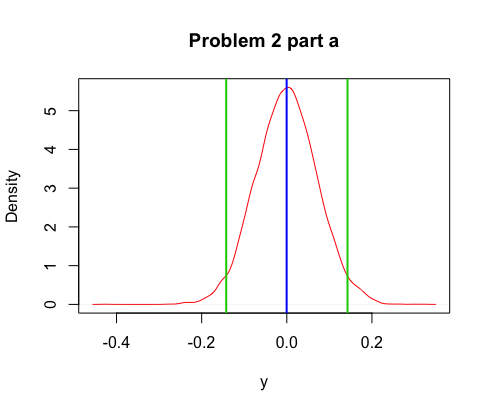
\includegraphics[width=6.5cm,height=6.5cm,keepaspectratio]{P2a1}
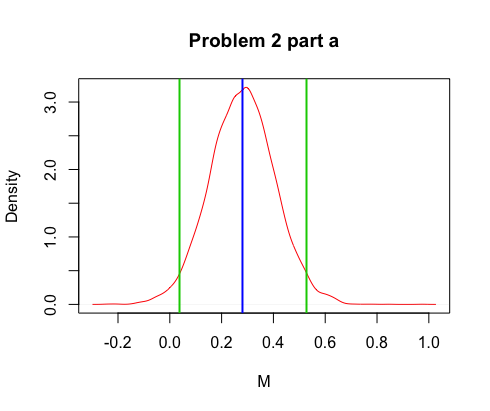
\includegraphics[width=6.5cm,height=6.5cm,keepaspectratio]{P2a2}\\
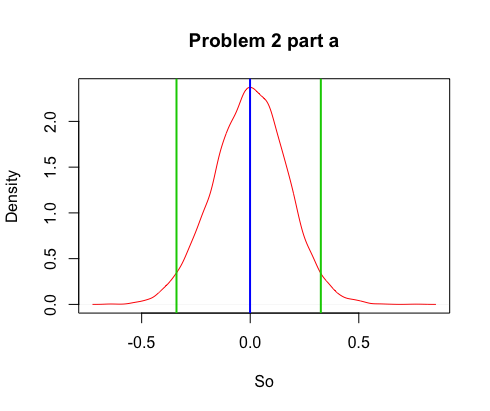
\includegraphics[width=6.5cm,height=6.5cm,keepaspectratio]{P2a3}
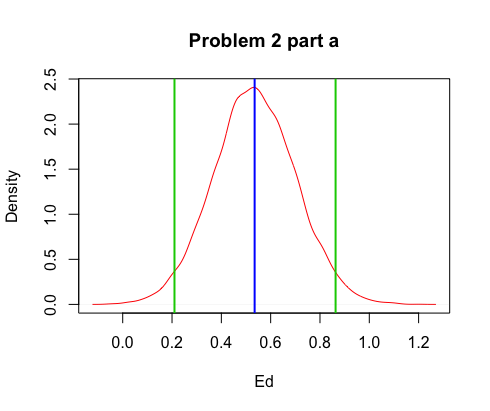
\includegraphics[width=6.5cm,height=6.5cm,keepaspectratio]{P2a4}\\
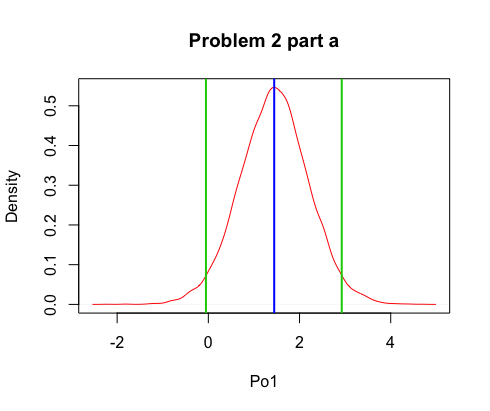
\includegraphics[width=6.5cm,height=6.5cm,keepaspectratio]{P2a5}
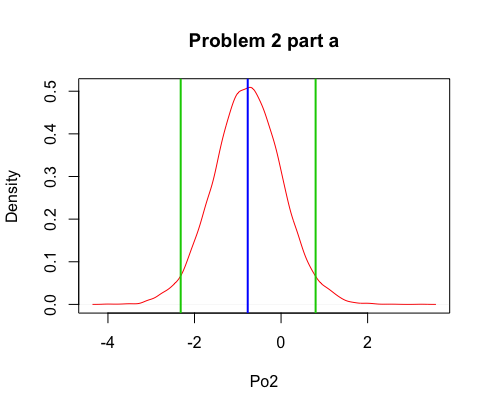
\includegraphics[width=6.5cm,height=6.5cm,keepaspectratio]{P2a6}\\
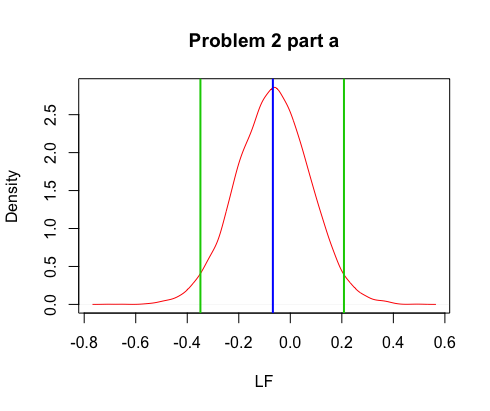
\includegraphics[width=6.5cm,height=6.5cm,keepaspectratio]{P2a7}
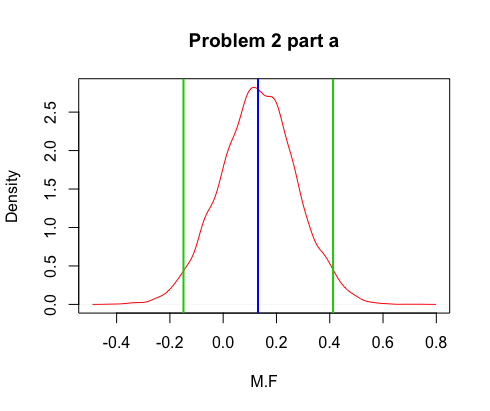
\includegraphics[width=6.5cm,height=6.5cm,keepaspectratio]{P2a8}\\
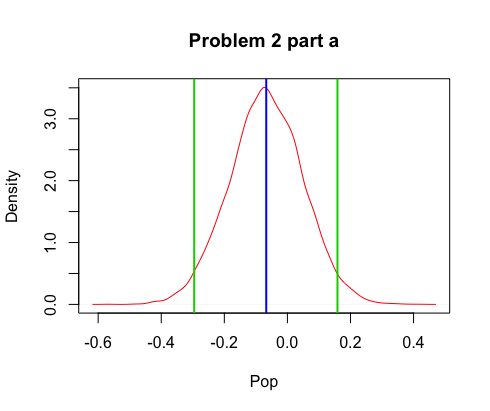
\includegraphics[width=6.5cm,height=6.5cm,keepaspectratio]{P2a9}
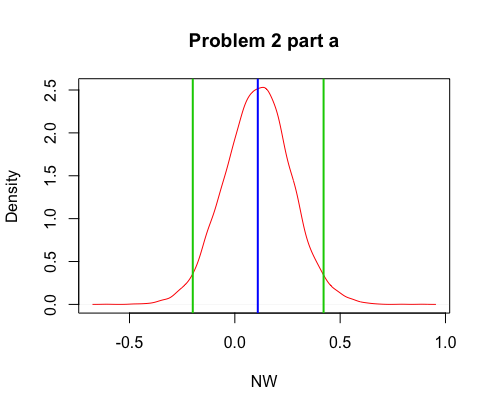
\includegraphics[width=6.5cm,height=6.5cm,keepaspectratio]{P2a10}\\
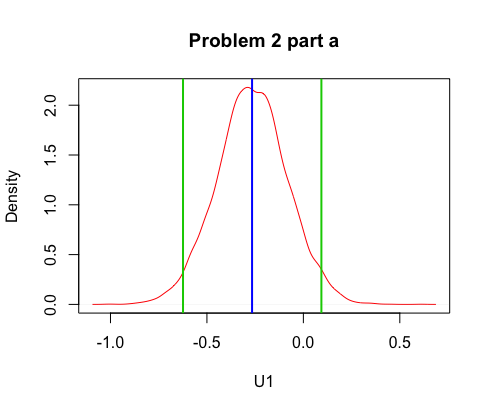
\includegraphics[width=6.5cm,height=6.5cm,keepaspectratio]{P2a11}
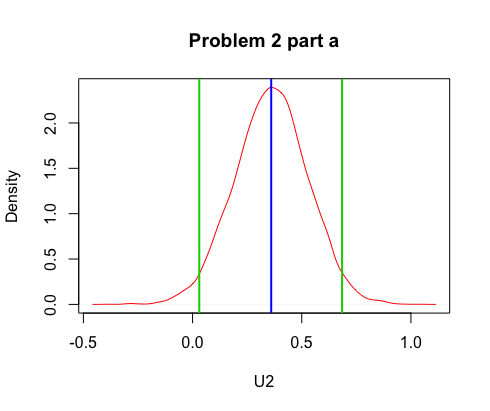
\includegraphics[width=6.5cm,height=6.5cm,keepaspectratio]{P2a12}\\
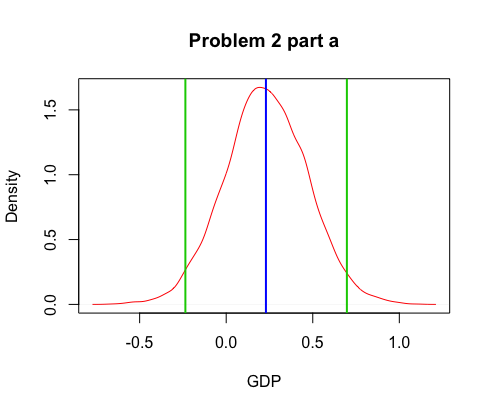
\includegraphics[width=6.5cm,height=6.5cm,keepaspectratio]{P2a13}
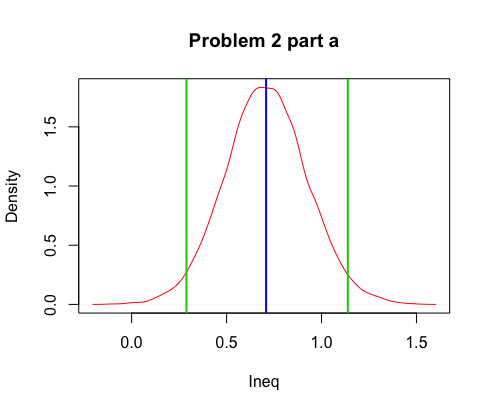
\includegraphics[width=6.5cm,height=6.5cm,keepaspectratio]{P2a14}\\
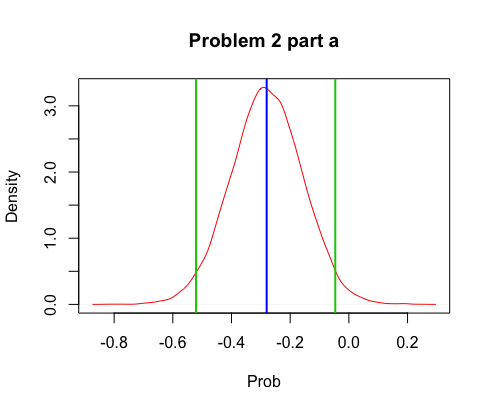
\includegraphics[width=6.5cm,height=6.5cm,keepaspectratio]{P2a15}
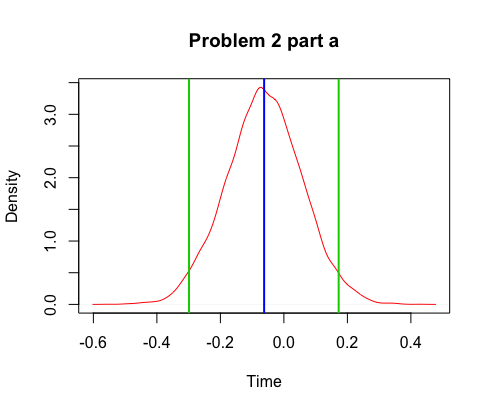
\includegraphics[width=6.5cm,height=6.5cm,keepaspectratio]{P2a16}\\
\end{center}


\begin{flushleft}
\textbf{Part b (i)}
\end{flushleft}
After randomly dividing the data into training and test data sets, we compute $\hat{y_{ols}}$ and subsequently plot it against $y_{te}$ (below). The prediction error was found to be 0.5562. 
\\
\\\
\textit{R code and output on the next page}\\
\newpage
\textbf{R Code} 
\\\
\lstset{backgroundcolor=\color{light-gray}, frame=single, basicstyle = \ttfamily\small}
\begin{lstlisting}{language=R}
> #Problem 2 Part b (i)
> 
> set.seed(1)
> tr = sample(1:n, n/2)
> te = (1:n)[-tr]
> X_tr = X[tr,]
> X_te = X[te,]
> y_tr = y[tr,]
> y_te = y[te,]
> beta_ols = solve(t(X_tr)%*%X_tr)%*%t(X_tr)%*%y_tr
> y_ols = X_te%*%beta_ols
> dev.off()
> plot(y_te, y_ols, xlab = "y_te", ylab = "y_ols", 
main='Problem 2 part b (i)', xlim = c(-2, 4), ylim = c(-2, 4), 
asp = 1);
> abline(c(0, 0), c(1, 1), col = "red")
> sum((y_ols-y_te)^2)/length(y_te)
[1] 0.5562224
\end{lstlisting} 
\textbf{Plot:} \\
\begin{center}
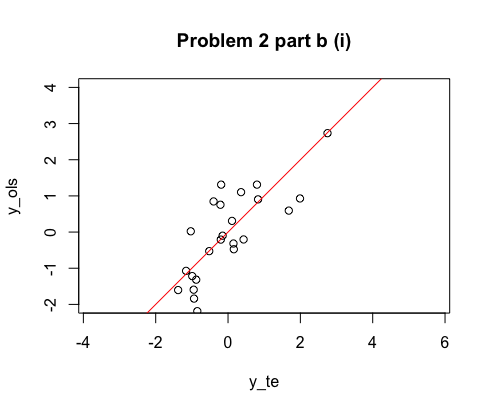
\includegraphics[width=9cm,height=9cm,keepaspectratio]{2bi.png}
\end{center}
\begin{flushleft}
\textbf{Part b (ii)}
\end{flushleft}
Now we are going to use the g-prior from part a and use only the training set to compute $\hat{y_{Bayes}}$. Then we plot versus the test data (below). The prediction error was found to be 0.5219, which is smaller than the OLS prediction error determined in part a. 
\\
\\\
\textit{R code and output on the next page}\\
\textbf{R Code} 
\\\
\lstset{backgroundcolor=\color{light-gray}, frame=single, basicstyle = \ttfamily\small}
\begin{lstlisting}{language=R}
> #Problem 2 Part b (ii)
> 
> g = length(y_tr);
> nu_0 = 2;
> sigma2_0 = 1;
> n = dim(X_tr)[1];
> m = dim(X_tr)[2];
> t = 10000;
> Hg = (g/(g+1))*X_tr%*%solve(t(X_tr)%*%X_tr)%*%t(X_tr);
> SSR = t(y_tr)%*%(diag(1, nrow = n)-Hg)%*%y_tr;
> sigma2 = 1/rgamma(t, (nu_0+n)/2, (nu_0*sigma2_0+SSR)/2);
> Vb = g*solve(t(X_tr)%*%X_tr)/(g+1);
> Eb = Vb%*%t(X_tr)%*%y_tr;
> E = matrix(rnorm(t*m, 0, sqrt(sigma2)), t, m);
> beta_bayes = colMeans(t(t(E%*%chol(Vb))+c(Eb)));
> y_bayes = X_te%*%beta_bayes;
> plot(y_te, y_bayes, xlab = "y_te", ylab = "y_bayes", 
main='Problem 2 part b (ii)', xlim = c(-2, 4), ylim = c(-2, 4), 
asp = 1);
> abline(c(0, 0), c(1, 1), col = "red");
> sum((y_bayes-y_te)^2)/length(y_te);
[1] 0.5218922
\end{lstlisting} 
\textbf{Plot:} \\
\begin{center}
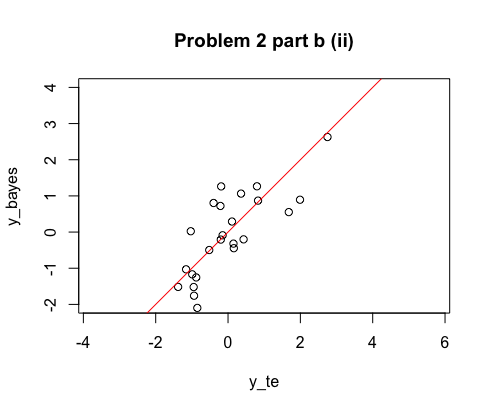
\includegraphics[width=9cm,height=9cm,keepaspectratio]{2bii.png}
\end{center}
\newpage
\begin{flushleft}
\textbf{Part c}
\end{flushleft}
The above procedures in part b were repeated 10,000 times and an average prediction error was subsequently computed for the OLS method and was found to be 1.2162 . Using Bayesian methods, the average prediction error was found to be 1.1456. Again, we see that the average prediction error when implementing Bayesian methods is lower throughout 10000 randomly generated test sets. 
\\
\textit{R code and output below}\\
\\\
\textbf{R Code} 
\\\
\lstset{backgroundcolor=\color{light-gray}, frame=single, basicstyle = \ttfamily\small}
\begin{lstlisting}{language=R}
> #Problem 2 part c
> t1 = 10000;
> error_ols = rep(NA, 1, t1);
> error_bayes = rep(NA, 1, t1);
> for (i in 1:t1) {
+     set.seed(i);
+     n = 47;
+     tr = sample(1:n, n/2);
+     te = (1:n)[-tr];
+     X_tr = X[tr,];
+     X_te = X[te,];
+     y_tr = y[tr,];
+     y_te = y[te,];
+     beta_ols = solve(t(X_tr)%*%X_tr)%*%t(X_tr)%*%y_tr;
+     y_ols = X_te%*%beta_ols;
+     error_ols[i] = sum((y_ols-y_te)^2)/length(y_te)
+     g = length(y_tr);
+     nu_0 = 2;
+     sigma2_0 = 1;
+     n = dim(X_tr)[1];
+     m = dim(X_tr)[2];
+     t = 10000;
+     Hg = (g/(g+1))*X_tr%*%solve(t(X_tr)%*%X_tr)%*%t(X_tr);
+     SSR = t(y_tr)%*%(diag(1, nrow = n)-Hg)%*%y_tr;
+     sigma2 = 1/rgamma(t, (nu_0+n)/2, (nu_0*sigma2_0+SSR)/2);
+     Vb = g*solve(t(X_tr)%*%X_tr)/(g+1);
+     Eb = Vb%*%t(X_tr)%*%y_tr;
+     E = matrix(rnorm(t*m, 0, sqrt(sigma2)), t, m);
+     beta_bayes = colMeans(t(t(E%*%chol(Vb))+c(Eb)));
+     y_bayes = X_te%*%beta_bayes;
+     error_bayes[i] = sum((y_bayes-y_te)^2)/length(y_te);
+   }
> mean(error_ols)
[1] 1.216266
> mean(error_bayes)
[1] 1.145592
\end{lstlisting}
\end{problem}

\begin{problem}{3} \textit{Problem 10.2 from Hoff}\\
\\\
\textbf{Part a}
\\\
We know that $Y_{i}$ is a binary indicator r.v. corresponding to whether or not the $i^{th}$ sparrow successfully nests, so we have that \\
$$p(y_{i}|\alpha,\beta,x_{i})=p_{i}^{y_{i}}(1-p_{i})^{1-y_{i}}$$
The joint sampling distribution is then\\
$$\prod_{i=1}^{n} p(y_{i}|\alpha,\beta,x_{i})=\prod_{i=1}^{n}p_{i}^{y_{i}}(1-p_{i}^{1-y_{i}})\\
=\prod_{i=1}^{n} exp\left\lbrace y_{i}log(\frac{p_{i}}{1-p_{i}})+log(1-p_{i})\right\rbrace\\
$$ $$ = \ exp\left\lbrace \sum_{i=1}^{n}y_{i}log(\frac{p_{i}}{1-p_{i}})+\sum_{i=1}^{n}log(1-p_{i})\right\rbrace$$\\
Since we are using the logit link, \ $log(\frac{p_{i}}{1-p_{i}})=\alpha+\beta x_{i}$, we have
$$\prod_{i=1}^{n}p(y_{i}|\alpha,\beta,x_{i})=exp\left\lbrace\sum_{i=1}^{n}y_{i}(\alpha+\beta x_{i})-\sum_{i=1}^{n}log(1+exp(\alpha+\beta x_{i}))\right\rbrace$$\\
\\\
\textbf{Part b}
\\\
Using logistic regression, we can determine the prior distributions for $\alpha$ and $\beta$ as follows \\
\textit{R code below}\\
$$ \alpha \sim N(\mu_{\alpha},\sigma_{\alpha}^{2}), \ where \ \mu_{\alpha}=-9.78681, \ \sigma_{\alpha}=4.620189$$
$$\beta \sim N(\mu_{\beta},\sigma_{\beta}^{2}), \ where \ \mu_{\beta}=0.7757703, \ \sigma_{\beta}=0.3578308$$
\textbf{R Code}
\lstset{backgroundcolor=\color{light-gray}, frame=single, basicstyle = \ttfamily\small}
\begin{lstlisting}{language=R}
#Problem 3 Part b
msparrownest <- read.table("msparrownest.dat", quote="\"",
 comment.char="")
y=msparrownest$V1
x=msparrownest$V2
f1=glm(formula = y~x,family = binomial, data=msparrownest)
mu.alpha=summary(f1)$coefficients[1,1]
mu.alpha
sd.alpha=summary(f1)$coefficients[1,2] 
sd.alpha
mu.beta=summary(f1)$coefficients[2,1]
mu.beta
sd.beta=summary(f1)$coefficients[2,2]
sd.beta
\end{lstlisting}
\newpage
\begin{flushleft}
\textbf{Part c}
\end{flushleft}
A Metropolis algorithm was implemented using $10^{7}$ repetitions using the R code below. We achieved an acceptance rate of 0.3003839. The effective sample size for $\alpha$ is 1,055 and the effective sample size for $\beta$ is 1,107,  so both are greater than 1,000, as desired. \\
\\\
\textbf{R Code}
\lstset{backgroundcolor=\color{light-gray}, frame=single, basicstyle = \ttfamily\small}
\begin{lstlisting}{language=R}
#Problem 3 Part c
posterior=function(alpha,beta,y,x){
  b=sum(log(1+exp(alpha+beta*x))) 
  theta=alpha+beta*x
  likelihood=exp(sum(y*theta)-b)
  prior.alpha=dnorm (alpha, mean=mu.alpha, sd=sd.alpha)
  prior.beta=dnorm (beta, mean=mu.beta, sd=sd.beta)
  return(likelihood*prior.alpha*prior.beta)
}
#Metropolis   
B=20000
n=10000000
alpha.m=rep(NA,B+n)
beta.m=rep(NA,B+n)
alpha.m[1]=mu.alpha
beta.m[1]=mu.beta
acc=0
for ( t in 2:(B+n)){
  alpha.new=rnorm(1,mean=alpha.m[t-1],sd=.1)
  beta.new=rnorm(1,mean=beta.m[t-1],sd=.1) 
  pi.new=posterior(alpha.new, beta.new, y,x)
  pi.t=posterior(alpha.m[t-1], beta.m[t-1], y,x) 
  rho=min(c(pi.new/pi.t,1))
  U=runif (1 ,min=0,max=1) 
  if (U<rho){
    alpha.m[t]=alpha.new
    beta.m[t]=beta.new
    acc=acc+1
} else{
  alpha.m[t]=alpha.m[t-1]
  beta.m[t]=beta.m[t-1]
}
}
print(acc/(B+n))
effectiveSize(alpha.m)
effectiveSize(beta.m[1:((B+n)/2)]) +
  effectiveSize(beta.m[((B+n)/2+1):(B+n)])
\end{lstlisting}
\newpage
\begin{flushleft}
\textbf{Part d}
\end{flushleft}
The posterior densities (black curve) and prior densities (blue curve) for $\alpha$ and $\beta$ were plotted in R (Plots below). Referring to the plots, we can see that the posterior and prior densities for both $\alpha$ and $\beta$ have significant differences. The posterior distributions have higher peaks and thinner tails compared to the prior distributions (as seen below), which was to be expected. However, it appears that they have roughly the same mean, for both  $\alpha$ and $\beta$. \\
\\\
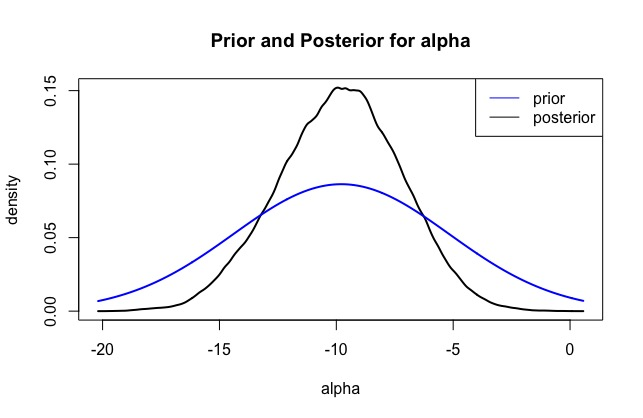
\includegraphics[width=3.5in]{3dalpha}
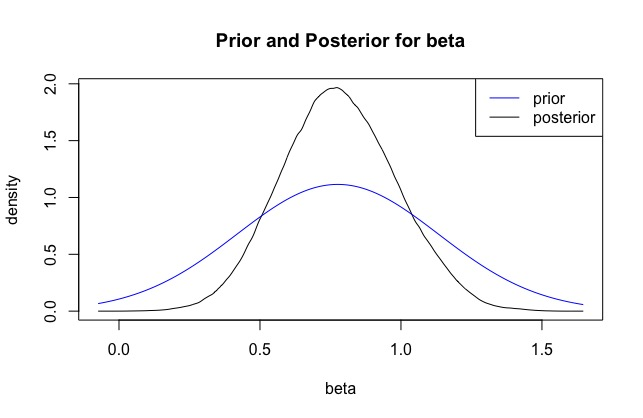
\includegraphics[width=3.5in]{3dbeta}\\
\textbf{R Code}
\lstset{backgroundcolor=\color{light-gray}, frame=single, basicstyle = \ttfamily\small}
\begin{lstlisting}{language=R}
#Problem 3 Part d
grapha=density(alpha.m)
graphb=density(beta.m)
prior.alpha=dnorm(grapha$x, mean=mu.alpha, sd=sd.alpha)
prior.beta=dnorm(graphb$x, mean=mu.beta, sd=sd.beta)
plot(grapha$x,grapha$y,lwd=2,typ="l", xlab = "alpha", 
     ylab = "density", main = "Prior and Posterior for alpha")
lines(grapha$x,prior.alpha,col="blue",lwd=2)
legend("topright",legend = c("prior","posterior"),lwd=c(1,1), 
       col=c("blue","black"))
plot(graphb$x,graphb$y,typ="l",xlab = "beta",ylab = "density", 
     main = "Prior and Posterior for beta")
lines(graphb$x,prior.beta,col="blue")
legend("topright",legend = c("prior","posterior"),lwd=c(1,1), 
       col=c("blue","black"))
\end{lstlisting}
\newpage
\begin{flushleft}
\textbf{Part e}\\
\end{flushleft}
A 95\% confidence band for the given function $f_{\alpha\beta}(x)$  of wingspan is given below\\
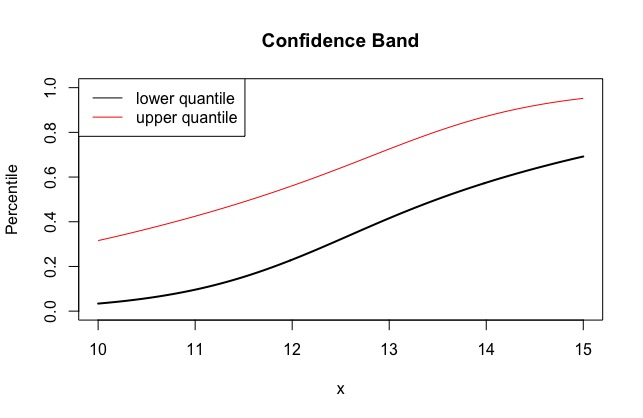
\includegraphics[width=5in]{3e}\\
\textbf{R Code}
\lstset{backgroundcolor=\color{light-gray}, frame=single, basicstyle = \ttfamily\small}
\begin{lstlisting}{language=R}
#Problem 3 Part e
x.seq=seq(10,15,by=0.02) 
conf.band=matrix(NA,nrow=length(x.seq),ncol=2) 
for (i in 1:length(x.seq)) {
  fun=exp(alpha.m+beta.m*x.seq[i])
  fun1=fun/(1+fun) 
  conf.band[i,]=quantile(fun1,probs=c(0.025, 0.975), na.rm = TRUE) 
}
plot(x.seq,conf.band[,1],ylim=c(0,1),lwd=2,col="black",type="l", 
     main="Confidence Band",xlab="x",ylab="Percentile")
points(x.seq,conf.band[,2],col="red",type="l")
legend("topleft", col=c("black","red"), 
       legend=c("lower quantile","upper quantile"), lwd = c(1,1))
\end{lstlisting}
\end{problem}

\begin{problem}{4}
\text{} \\
\textbf{Part 1}\\
We first compute the conditional distributions as follows:\\
 $$\beta|rest \sim MVN\left(\left(\frac{I}{100}+\frac{X^T X}{\sigma^2}\right)^{-1}\frac{X^T z}{\sigma ^2},  \ \ \left(\frac{I}{100}+\frac{X^T X}{\sigma^2}\right)^{-1}\right) $$\\
 $$p(z_i|rest)\propto exp[y_i z_i-log(1+e^{z_i})-\frac{1}{2\sigma^2}(z_i-x_i^T \beta)^2] ~\ i=1,2,...,n$$\\
We now set $\sigma^2=1$ and apply Metropolis Hastings algorithm. The R code and the output/results are given below.\\
\lstset{backgroundcolor=\color{light-gray}, frame=single, basicstyle = \ttfamily\small}
\begin{lstlisting}{language=R}
#Problem 4 Part 1
library(LearnBayes)
library(MASS)
data(donner)

y=as.matrix(donner$survival,ncol=1)
X=cbind(1,donner$age,donner$male)
n=dim(X)[1]
p=dim(X)[2]
X=as.matrix(X,nrow=n,ncol=p)
Sigma=solve(diag(x=1,nrow=p,ncol=p)/100+t(X) %*% X)
#Gibbs 
B=1000
nmc=10000
beta.mc=matrix(NA,nrow=p,ncol=nmc+B)
z.mc=matrix(NA,nrow=n,ncol=nmc+B)
fit.freq=glm(donner$survival~X-1,family=binomial)
beta.mc[,1]=fit.freq$coefficients
z.mc[,1]=X%*%beta.mc[,1]
zi.cond<-function(zi,xi,beta,sigma,yi){
  a=dnorm(zi,mean=t(xi)%*%beta,sd=sigma)*exp(yi*zi-log(1+exp(zi)))
  return(a)
}

for (t in 2:(B+nmc)){
  mu.beta=Sigma %*% t(X) %*% as.matrix(z.mc[,t-1],ncol=1)
  beta.mc[,t]=mvrnorm(1,mu=mu.beta,Sigma)
  pz.s=mvrnorm(1,mu=z.mc[,t-1],Sigma=diag(x=1,nrow=n,ncol=n))
  for (i in 1:n){
    xi=as.matrix(X[i,],ncol=1)
    beta=as.matrix(beta.mc[,t],ncol=1)
    yi=y[i]
    pz.s=zi.cond(pz.s[i],xi,beta,sigma=1,yi)
    pz.t=zi.cond(z.mc[i,t-1],xi,beta,sigma=1,yi)
    rho=min(c(1,pz.s/pz.t))
    if (runif(1,min=0,max=1)<rho)
    { z.mc[i,t]=pz.s[i]
    }else{
      z.mc[i,t]=z.mc[i,t-1]
    }
  }
}

#Posterior results for logistic model
beta.mc=beta.mc[,(B+1):(B+nmc)]
beta.mc1.mean=apply(beta.mc,1,mean)
beta.mc1.lower=apply(beta.mc,1,quantile,.025)
beta.mc1.upper=apply(beta.mc,1,quantile,.975)
print(beta.mc1.mean)
print(beta.mc1.upper)
print(beta.mc1.lower)

#Probit model Results
beta.probit=bayes.probit(y,X,m=(nmc+B),prior=list(beta=c(0,0,0), 
P=diag(x=1,nrow=p,ncol=p)/100))$beta
beta.probit=beta.probit[(B+1):(B+nmc),]
beta.probit.mean=apply(beta.probit,2,mean)
beta.probit.lower=apply(beta.mc,1,quantile,.025)
beta.probit.upper=apply(beta.mc,1,quantile,.975)
print(beta.probit.mean)
print(beta.probit.upper)
print(beta.probit.lower)
\end{lstlisting}

The results of logistic posterior means and credible intervals for $\beta$ are given in the table below:\\

  \begin{center}
  \begin{tabular}{ |c|c|c|c| }
  \hline
  ~\ & Mean & Lower 2.5\% quantiles & Upper 2.5\% quantiles  \\ 
  Intercept & 4.1656533 & 1.2234501 & 8.05297357  \\ 
  \texttt{Age} & -0.1039775 & -0.2035014 & -0.02211799  \\
  \texttt{Male} & -1.9720865 & -4.0257651 & -0.25426965  \\
  \hline
  \end{tabular}
  \end{center}
  
The results of probit regression are summarized in the table below:\\ 
  \begin{center}
  \begin{tabular}{ |c|c|c|c| }
  \hline
  ~\ & mean & lower 2.5\% quantiles & upper 2.5\% quantiles  \\ 
  Intercept & 2.05396256 & 1.2234501 & 8.05297357  \\ 
  \texttt{Age} & -0.04961277 & -0.2035014 & -0.02211799  \\
 \texttt{Male} & -0.98946242 & -4.0257651 & -0.25426965  \\
  \hline
  \end{tabular}
  \end{center}
 
It is seen that the posterior means for $\beta$ are significantly different between the two models.\\
\\\
\textbf{Part 2}
\\\
First consider all of the conditionals, including the new conditional for $\sigma^2$:\\
$\beta|rest \sim MVN\left(\left(\frac{I}{100}+\frac{X^T X}{\sigma^2}\right)^{-1}\frac{X^T z}{\sigma ^2}, \left(\frac{I}{100}+\frac{X^T X}{\sigma^2}\right)^{-1}\right)  $\\
\\\
$ p(z_i|rest)\propto exp[y_i z_i-log(1+e^{z_i})-\frac{1}{2\sigma^2}(z_i-x_i^T \beta)^2] ~\ i=1,2,...,n$\\
\\\
$\sigma^2|rest \sim Inv-Gamma(a+\frac{n}{2}, \ b+\frac{1}{2}(z-X\beta)^T(z-X\beta)), ~\ where ~\ z=(z_1,...z_n)^T $\\
\\\
The R code and the results of logistic posterior means and credible intervals for $\beta$ are given below. \\
\\\
\textbf{R Code}
\lstset{backgroundcolor=\color{light-gray}, frame=single, basicstyle = \ttfamily\small}
\begin{lstlisting}{language=R}
#Problem 4 Part 2
B=2000
nmc=20000
beta.mc=matrix(NA,nrow=p,ncol=nmc+B)
z.mc=matrix(NA,nrow=n,ncol=nmc+B)
beta.mc[,1]=fit.freq$coefficients
z.mc[,1]=X%*%beta.mc[,1]
sigma2.mc=rep(NA,B+nmc)
sigma2.mc[1]=1
count=rep(0,n)

#Gibbs Sampling:
for (t in 2:(B+nmc)){
  Sigma.beta=solve(diag(x=1,nrow=p,ncol=p)/100+t(X) %*% 
  X/sigma2.mc[t-1])
  mu.beta=Sigma.beta %*% t(X) %*%as.matrix(z.mc[,t-1], 
  ncol=1)/sigma2.mc[t-1]
  beta.mc[,t]=mvrnorm(1,mu=mu.beta,Sigma.beta)
  pz.s=mvrnorm(1,mu=z.mc[,t-1],Sigma=0.01*diag(1,ncol=n,nrow=n))
  for (i in 1:n){
    xi=as.matrix(X[i,],ncol=1)
    beta=as.matrix(beta.mc[,t],ncol=1)
    yi=y[i]
    pz.s=zi.cond(pz.s[i],xi,beta,sigma=sqrt(sigma2.mc[t-1]),yi)
    pz.t=zi.cond(z.mc[i,t-1],xi,beta,sigma=sqrt(sigma2.mc[t-1]),yi)
    rho=min(c(1,pz.s/pz.t))
    if (runif(1,min=0,max=1)<rho){
      z.mc[i,t]=pz.s[i]
      count[i]=count[i]+1
    }
    else{z.mc[i,t]=z.mc[i,t-1]}
  }
  SSR.t = sum((z.mc[,t] - X %*% as.matrix(beta.mc[,t],ncol=1))^2)
  sigma2.mc[t] = 1/rgamma(1,shape=0.1+n/2,rate=1+SSR.t/2)
}
beta.mc=beta.mc[,(B+1):(B+nmc)]

#Posterior results for logistic model
beta.mc2.mean=apply(beta.mc,1,mean)
beta.mc2.upper=apply(beta.mc,1,quantile,.975)
beta.mc2.lower=apply(beta.mc,1,quantile,.025)
print(beta.mc2.mean)
print(beta.mc2.upper)
print(beta.mc2.lower)

#Probit model Results
beta.probit=bayes.probit(y,X,m=(nmc+B),prior=list(beta=c(0,0,0), 
P=diag(x=1,nrow=p,ncol=p)/100))$beta
beta.probit=beta.probit[(B+1):(B+nmc),]
beta.probit.mean=apply(beta.probit,2,mean)
beta.probit.upper=apply(beta.mc,1,quantile,.975)
beta.probit.lower=apply(beta.mc,1,quantile,.025)
print(beta.probit.mean)
print(beta.probit.upper)
print(beta.probit.lower)
\end{lstlisting}
 
 \begin{center}
  \begin{tabular}{ |c|c|c|c| }
  \hline
  ~\ & mean & lower 2.5\% quantiles & upper 2.5\% quantiles  \\ 
  Intercept & 4.633564 & 1.721778 & 7.54241823  \\ 
  \texttt{Age} & -0.111619 & -0.184988 & -0.03621309  \\
  \texttt{Male} & -2.471943 & -4.656946 & -0.45278008  \\
  \hline
  \end{tabular}
 \end{center}
 
The results of probit regression:\\ 
 \begin{center}
  \begin{tabular}{ |c|c|c|c| }
  \hline
  ~\ & mean & lower 2.5\% quantiles & upper 2.5\% quantiles  \\ 
  Intercept &  2.05353078 & 1.721778 & 7.54241823  \\ 
  \texttt{Age} & -0.04951136 & -0.184988 & -0.03621309  \\
  \texttt{Male} & -0.99562403 & -4.656946 & -0.45278008  \\
  \hline
  \end{tabular}
 \end{center}
 
While the results from Part 1 and Part 2 are similar,  the two models produce significantly different posterior means.   \\

\end{problem}

\begin{problem}{5}
\text{ }\\
\textbf{1.} \ We are given that $Y_i\sim Poisson(\lambda_i)$, so\\
$$p(y_{i}|\lambda_{i})=exp(-\lambda_{i})\frac{\lambda_{i}^{y_{i}}}{y_{i}!}=exp\left\lbrace y_{i}log \lambda_{i}-\lambda_{i}-log(y_{i}!)\right\rbrace$$
From the above it is seen that the canonical link is $\theta_{i}=log \lambda_{i}$.\\
Using this canonical link, $\theta_{i}=\eta_{i}=x_{i}^{T}\beta=log(\lambda_{i}) \ \Longrightarrow \ \lambda_{i}=exp(x_{i}^{T} \beta)$\\
Plugging this into the conditional density, we get\\
$$p(y_{i}|x_{i}, \beta)=exp\left\lbrace y_{i}x_{i}^{T} \beta -log(y_{i}!)-exp(x_{i}^{T} \beta)\right\rbrace$$
Then the likelihood can be computed as follows \\
$$p(y|x, \beta)=\prod_{i=1}^{n}p(y_{i}|x_{i},\beta)\\
=exp\left\lbrace\sum_{i=1}^{n} y_{i}x_{i}^{T} \beta -\sum_{i=1}^{n}log(y_{i}!)-\sum_{i=1}^{n} exp(x_{i}^{T} \beta)\right\rbrace$$
\textbf{2.} \  Using the logit link instead, we get $\theta_{i}=log(\lambda_{i})=log(\eta_{i})=log(x_{i}^{T}\beta)$\\
$\Longrightarrow \ \lambda_{i}=x_{i}^{T}\beta$.\\
Plugging this into the conditional density:\\
$$p(y_{i}|x_{i},\beta)=exp(y_{i}log(x_{i}^{T}\beta)-log(y_{i}!)-x_{i}^{T}\beta)$$
The likelihood is then computed as follows: \\
$$p(y|x, \beta)=\prod_{i=1}^{n}p(y_{i}|x_{i},\beta)\\
=exp\left\lbrace \sum_{i=1}^{n} y_{i} log(x_{i}^{T} \beta) -\sum_{i=1}^{n}log(y_{i}!)-\sum_{i=1}^{n} x_{i}^{T} \beta\right\rbrace$$

\end{problem}


\end{document}